\documentclass{article}

\usepackage[T2A]{fontenc}
\usepackage[utf8]{inputenc}
\usepackage[english,russian]{babel}
\usepackage{mathtools}
\usepackage{cancel}
\usepackage[normalem]{ulem}
\usepackage{graphicx}%Вставка картинок правильная
\usepackage{wrapfig}%Обтекание фигур (таблиц, картинок и прочего)
\title{Название}
\author{Даня Грозный}
%\with{Владимир Владимирович}

\begin{document}
\section{Унификация разнородной задачи}
Чем более массовый алгоритм, тем лучше.

Множества $X$ кодируется с помощью $\Sigma*$ "--- множества всех слов алфавита $\Sigma$. 

$\forall x \in X \; x \to f(x) \in \Sigma*$.

Подмножества множества всех слов $L \subset \Sigma*$ "--- языки над алфавитом $\Sigma$.

\begin{figure}[h!]
    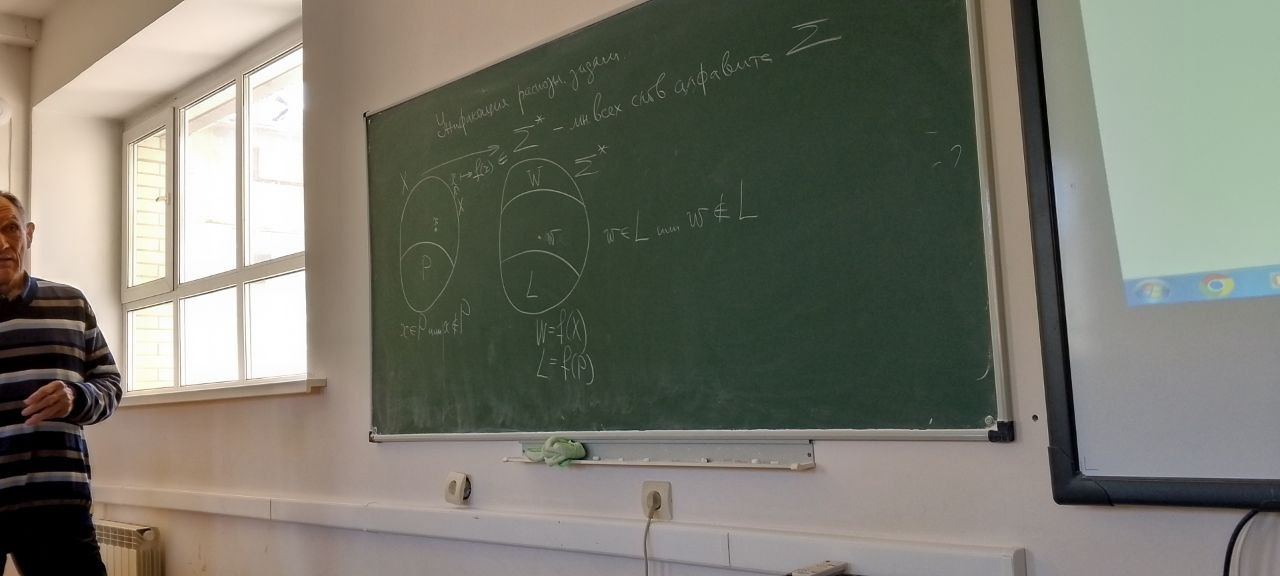
\includegraphics[width=\textwidth]{1.jpg}
\end{figure}

\begin{figure}[h!]
    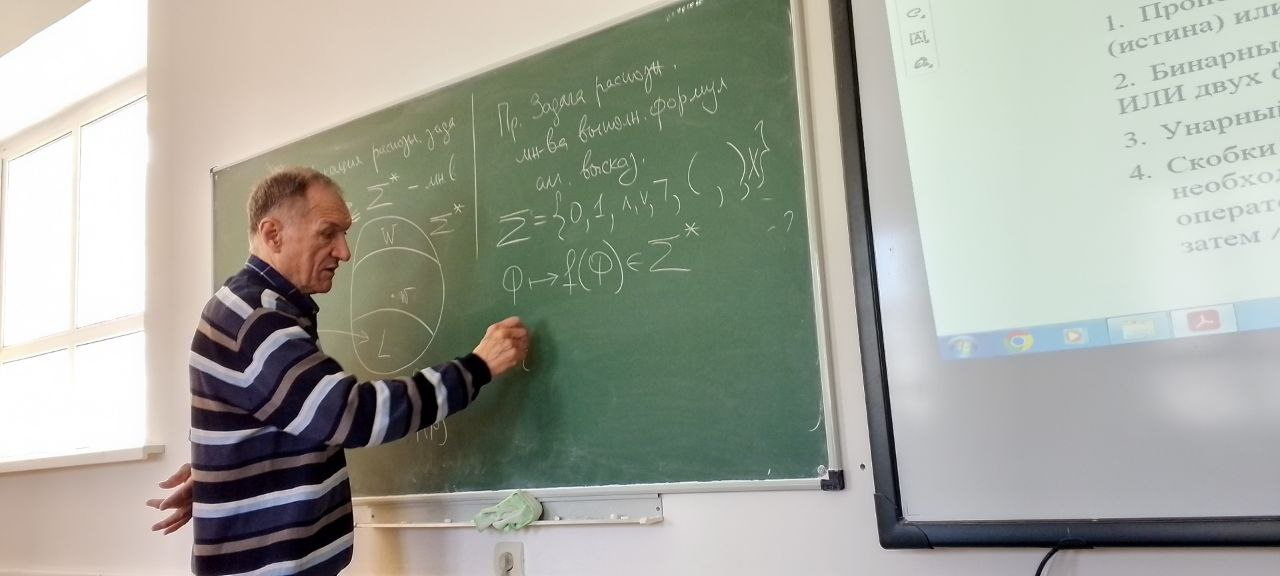
\includegraphics[width=\textwidth]{2.jpg}
\end{figure}

$X_i \to X[i]_z \in \Sigma*$

$L = \{f(\varphi) : \varphi \, \text{ --- выполнимая формула}\}$

$W \in f(\text{Г}_{AB})$

\subsection{Интуитивное понятие алгоритма и его математические модели.}

Под алгоритмом интуитивно понимается совокупность инструкицй, которые дают решение некоторой массовой задачи.

Общие свойства алгоритма:

\begin{enumerate}
    \item дискретность алгоритма
    \item детерминированность алгоритма
    \item элементарность шагов алгоритма
    \item массовость алгоритма
\end{enumerate}

Множество слов для алфавита $\Sigma = \{0,1\}$ имеет вид:
\begin{equation}
    \Sigma* = \{\land, 0, 1, 00, 01, 10, 11, \dots\},
\end{equation}
где $\land$ "--- пустое слово (его наличие подразумевается, когда множество слов обозначается символом $*$).

Алгоритмически неразрешимые задачи привели к необходимости строго математического определения алгоритма.

Основные варианты математического определения алгоритма "--- модели алгоритма:
\begin{enumerate}
    \item понятие рекурсивной функции, введённое в 1936 году
    \item понятие машины Тьюринга, введённое Постом и Тьюрингом в 1936 году
    \item понятие нормального алгорифма, введённое Марковым в 1954 году
    \item понятие формальной грамматики, введённое Хомским в 1957 году
\end{enumerate}

\subsection{Машины Тьюринга}
\subsubsection{Логическое описание}
Реализация модели вычислений с помощью понятия машины Тьюринга.

При построении математической модели алгоритма Пост и Тьюрин исходили из того, что Молчанов пидорас заебал листать

Сщематическое описание работы машины Тьюринга:
\begin{figure}[h!]
    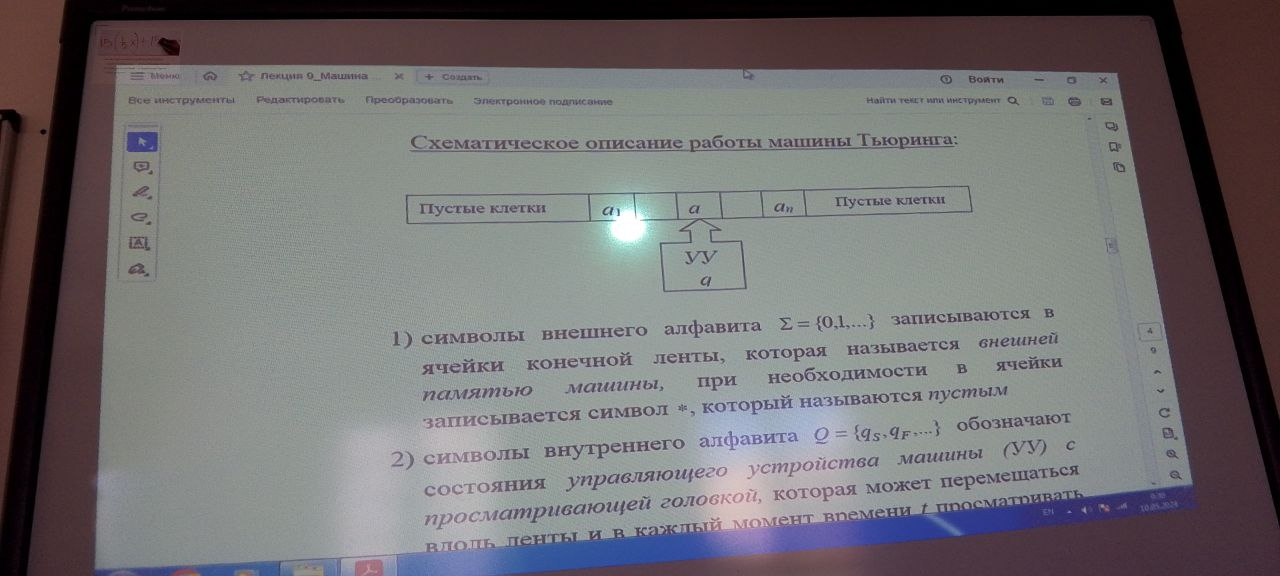
\includegraphics[width=\textwidth]{3.jpg}
\end{figure}
\begin{enumerate}
    \item символы внешнего алфавита $\Sigma$ записываются в ячейки конечной ленты, которая называется \textit{внешней памятью машины}, при необходимости в ячейки записывается символ *, который называется пустым
    \item символы внутреннего алфавита $Q = \{q_S, q_F, \dots\}$ обозначают состояния \textit{управляющего устройства машины (УУ) с просматривающей головкой}, которая может перемещаться вдоль ленты и в каждый момент времени $t$ просматривать одну ячейко,
    \item \textit{программа машины}
    \begin{equation}
        \Pi = \{T(q,a) : q \in Q \not \{q_F\} \land a \in \Sigma\}
    \end{equation}
    состоит из \textit{команд} $T(q, a) = qa \to q'a'X$, которые в зависимости от состояния машины $q$ и символа $a$ в просматриваемой ячейке УУ заменяют в этой ячейке букву $a$ на букву $a'$, состояние $q$ на состояние $q'$ и в зависимости от значения $X \in \{R, L, S\}$ сдвигают просматриваемую головку на месте при $X = S$. При необходимости на ленте достраиваются справа или слева ячейки с пустым символом $*$,
    \item машина начинает работать в \textit{начальном} состоянии $q_S$ и заканчивает работать в \textit{заключительном} состоянии $q_F$
    \item \underline{Вход машины}: слово $w \in \Sigma*$ на ленте машины $T$ в начальном состоянии $q_S$.

    \underline{Выход машины}: слово $w' \in \Sigma*$ на ленте машины $T$ в заключительном состоянии $q_F$
\end{enumerate}

Корректность заключается в том, что при заданном наборе входных данных мы должны достигать заключительного состояния. Однако не всегда это возможно.

В чём идельность машины Тьюринга? Лента внешней памяти потенциально бесконечна в обе стороны. Это причина, по которой машина Тьюринга нереализуема.

\subsubsection{Математическое описание машины Тьюринга}
\underline{Определение}. \textit{Машина Тьюринга} $T$ представляет собой алгебраическую систему $T=(\Sigma, Q, \delta, q_S, q_F)$, работающую в дискретные моменты времени $t=0,1,2,\dots$ и состояющую из следующих частей:
\begin{itemize}
    \item конечное множество $\Sigma=\{0,1,\dots\}$ --- внешний алфавит,
    \item конечное множество $Q = \{q_S, q_F, \dots\}$ --- внутренний алфавит, элементы Q называются \textit{состояниями машины},
    \item отображение $\delta: Q x E \to Q x \Sigma x \{R, L, S\}$, которое определяет список команд $T(q, a) = qa \to q'a'X$ --- символическое обозначение образов $\delta(q, a) = (q',a',X)$ отображения $\delta$ для $q \in Q \backslash \{q_F\}, a \in \Sigma$ и $X \in \{R, L, S\}$, множество всех команд Молчанов блять молчит очко разрабатывает
\end{itemize}

Работа машины Тьюринга $T$ происходит под действием её команд и заклчается в изменнии её \textit{конфигураций}, описывающих состояния ленты и управляющего устройства, а также положение головки относительно ячеек ленты:

если лента находится в состоянии, которое описывается словом $\alpha a \beta$ над алфавитом $\Sigma$, и головка в состоянии $q$ просматривает на ленте ячейку с состоянием $a$, то соответствующая конфигурация $K$ машины $T$ описывается выражением $M = \alpha q a  \beta$, которое называется \textit{машинным словом}.

При этом $K$ называется \textit{начальной конфигурацией}, если описывающее её машинное слово содержит символ начального состояния $q_S$, и \textit{заключительной конфигурацией}, если описывающее её машинное слово содержит символ заключительного состояния $q_F$.

Программа указывает, что делает в каждый момент времени в зависимости от её настоящей конфигруаиции $K$:

если $K$ --- заключительная конфигурация, то машина заканчивает работу, если же  $K$ не является заключительной кнофигурацией и описывается машинным словом $M = \alpha q a \beta$, то в программе $\Pi$  машина находит команду $T(q, a)$ с левой частью $qa$ и в зависимости от вида правой части такой команды $T(q, a)$ машина заменяет в просматриваемой ячейке букву $a$ на букву $a'$, сотояние $q$ на состояние $q'$ и в зависимости от значения $X \in \{R, L, S\}$ сдвигает просматривающую головку либо в соседнюю правую ячейку при $x = R$, либо в соседнюю левую ячейку при $X = L$, либо оставляет головку на месте при $X = S$.

Изменение конфигураций $K_0, K_1, K_2, \dots$ машины $T$ под действием команд происходит в дискретные моменты времени и описывается \\ $M_0, M_1, M_2, \dots$ по следующему правилу. За один шаг работы машины $T$ её машинное слово $M = \alpha q a \beta$ под действием команды $T(q, a)$ преобразуется в новое машинное слово $M'$ по формулам:

\begin{figure}[h!]
    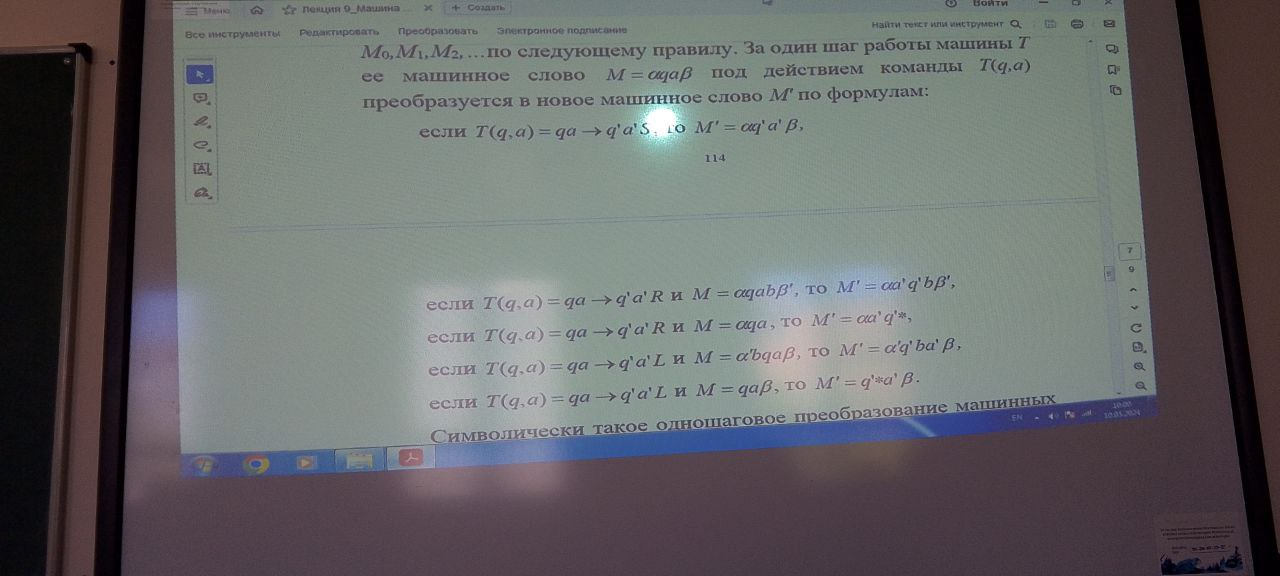
\includegraphics[width=\textwidth]{4.jpg}
\end{figure}

Символически эти одношаговые преобразования показывают преобразования машинных слов. Оно обозначается как $M \to^T M'$.

$\exists$ последовательность преобразований машинных слов $M \to^T M'$ (где $i = 0,1, \dots, k-1$), для которой $M_0 = M$, $M_k = M'$ $\Rightarrow$ пишут "$M \Rightarrow^T M'$"  и говорят, что \textit{машинное слово $M'$ получается из машинного слова $M$ с помощью машины $T$}.

\underline{Вход (начало работы ) машины}: слово $w \in \Sigma*$ на ленте машины $T$ в начальном состоянии $q_S$.

\underline{Выход (завершение работы) машины}: слово $w' \in \Sigma*$ на ленте машины $T$ в заключительном состоянии $q_F$.

В этом случае говорят, что машина $T$ \textit{принимает} слово $w$ и выдаёт знаение $w'=T(w)$. В результате машина $T$ определяет язык $L(T) \subset \Sigma*$, который состоит из всех принимаемых машиной $T$ слов.

\underline{Определение}. Язык $L \subset \Sigma*$ \textit{принимается} машиной Тьюринга, если $L = L(T)$ для некоторой машины Тьюринга $T$.

Таким образом, любая машина Тьюринга $T$ определяет частичную функцию $f$ из $\Sigma*$ и $\Sigma*$, область определения которой $D_f$ состоит из всех слов алфавита $\Sigma$, которые принимает машина $T$, и значения которой для слов $w \in D_f$ определяются по фромуле $f(w) = T(w)$. То есть не для всех слов машина достигает заключительного состояния.

\underline{Определение}. Частиная функция $f$ из $\Sigma*$ в $\Sigma*$ называется вычислимой по Тьюрингу, если она определяется некоторой машиной Тьюринга.

\underline{Пример}. Пусть машина Тьюринга $T$ имеет внешний алфавит $\Sigma = \{0,1\}$ внутренний алфавит $Q = \{q_S, q_F, q\}$ и программу $\Pi$, которая состоит и команд: (1)$q_S1 \to q1R$, (2) $q1 \to q1R$, (3) $q *\to q_F1S$. Тогда слово $\alpha = 11$ машиной $T$ перерабатывается в слово $\beta = 111$, так как
\begin{equation}
    \underline{q_s1}1 \underset{(1)}\to^T 1\underline{q1} \underset{(2)}\to^T 11\underline{q*} \underset{(3)}\to^T 11\underline{q_F}1 \; \text{и} \; T(11) = 111
\end{equation}

\underline{Основная теорема}. Для любой частичной словарной фукнции $f : (\Sigma*)^M \to \Sigma*$ следующие условия эквивалентны:
\begin{enumerate}
    \item функция $f$ вычислима по Тьюрингу
    \item функция $f$ частично рекурсивна
    \item функция $f$ нормально вычислима
\end{enumerate}

Задача называется \textit{алгоритмически разрешимой} или \textit{алгоритмически неразрешимой} в зависимости от того, есть или нет алгоритм решения этой задачи.

\section{Вычислимость: разрешимые и полуразрешимые языки}

\underline{Определение 1}. Язык $L$ называется \textit{разрешимым} (или \textit{рекурсивным}), если существует такая машина Тьюринга $T$, что для любого слова $w \in W$ выполняются условия:
\begin{itemize}
    \item если $w \in L$, то при входе $w$ машина $T$ попадает в заключительное состояние, останавливается и выдаёт значение $T(w) = 1$
    \item если $w \not \in L$, то при входе $w$ машина $T$ попадает в заключительное состояние, останавливаетс и выдаёт значение $T(w) = 0$
\end{itemize}

Такие машины соответствуют понятию <<алгоритма>> и применяются при решении \textit{распознавательных задач} типа <<да/нет>>.

Множество всех разрешимых языков будем обозначать $R$ (от Recursive).

\textbf{Свойства}: дополнения, конечные пересечения и конечные объединения разрешимыъх языков являются разрешимыми языками.

\textbf{Примеры разрешимых языков}.
\begin{itemize}
    \item Пустой языкМножество всех строк
    \item Конечные множества
    \item Множество чётных чисел
    \item Множество простых чисел
    \item Множество рациональных чисел, не превышающих $e$
    \item Множество всех чисел $n$, при которых в $\pi$ не меньше $n$ девяток подряд
\end{itemize}

\underline{Определение 2}. Язык $L$ называется \textit{полуразрешимым} или \textit{перечислимым}, если существует такая машина Тьюринга, что
\begin{equation}
    L = L(T) = \{w \in \Sigma* : T(w) = 1\},
\end{equation}
то есть при выходе $w \in L$ машина $T$ попадает в заключительное состояние, останавливается и выдаёт значение $T(w) = 1$, а при выходе $w \not \in L$\dots\dots\dots

\underline{Лемма}. Существуют неразрешимые языки, поскольку алгоритмов счётное число, а языков несчётное.

Аналогично можно доказать, что существуют языки, не являющиеся полуразрешимыми.

\underline{Основная теорема}. Существуют полуразрешимые неразрешимые языки, т. е. полуразрешимые языки, которые не могут быть разрешимы никакм алгоритмом, т. е. выполняется свойство $R \not \subset RE$.

\end{document}